\chapter[Additional Derivations and Formulae]{Additional Derivations and \\ Formulae}
\label{app:derivations}
\stoptocwriting
This appendix outlines further derivations and formulae used throughout this thesis.

\section{Ellipse Geometry}
\label{app:derivellipse}

Section \ref{s:trphysprop} considers the change in area when distorting a unit circle to an ellipse with the same circumference.
An ellipse can be defined in terms of the major and minor axis radii, denoted $a$ and $b$ respectively.
The distortion can then be described by the eccentricity, $\xi$, given by:
\begin{equation}
	\xi = \left(1-\frac{b^2}{a^2}\right)^{1/2}.
\end{equation}
The circumference of an ellipse of given eccentricity, $C\left(\xi\right)$, can then be calculated from the complete elliptic integral of the second kind,
\begin{equation}
	\label{eq:ellipsec}
	C\left(\xi\right) = 4a\int_0^{\pi/2} \left(1-\xi^2\sin^2\theta\right)^{1/2}\dd\theta,
\end{equation}
whilst the area is given more straightforwardly by
\begin{equation}
	A = \pi ab.
\end{equation}
The relative area between an ellipse and a unit circle for a given eccentricity is then
\begin{equation}
 	A/A^0=ab,
\end{equation} 
where $a$,$b$ satisfy $C\left(\xi\right)=2\pi$.

\section{Aboav\--Weaire with aG}
\label{app:derivag}

Section \ref{s:toptmapconfigspace} considers the meaning of the \aw{} parameter for aG systems \ie{} those containing just 5\--, 6\-- and 7\--rings.
For these relatively constrained systems, $\alpha$ can be related specifically to the proportions of specific ring adjacencies.
To derive this relationship, results are used from sections \ref{s:theorynodeprob} and \ref{s:toptmapconfigspace}.

The aG system has the node joint degree distribution
\begin{align}
	\mathbf{e} &= \begin{blockarray}{*{3}{c} l}
	\begin{block}{*{3}{>{$\footnotesize}c<{$}} l}
	5 & 6 & 7 \\
	\end{block}
	\begin{block}{[*{3}{c}]>{$\footnotesize}l<{$}}
	e_{55} & e_{56} & e_{57} \: \bigstrut[t]& 5\\
	e_{65} & e_{66} & e_{67} & 6 \\
	e_{75} & e_{76} & e_{77} & 7\\
	\end{block}
	\end{blockarray} .
\end{align}
Taking the \aw{} law, equation \eqref{eq:aboavweaire}, and noting that $m_5=\sumk ke_{5k}/q_5$, leads to the relationship
\begin{equation}
	\frac{5}{q_5}\left(5e_{55}+6e_{56}+7e_{57}\right) = \ki^2+\mu_2+\ki\left(1-\alpha\right)\left(5-\ki\right),
\end{equation}
to which several simplifications can be made.
These arise from the constraints $\ki=6$ and $\sumk e_{5k}=q_5$, which on substitution and rearrangement yield:
\begin{align}
	\frac{5}{q_5}\left(5e_{55}+6\left(q_5-e_{55}-e_{57}\right)+7e_{57}\right) &= 36+\mu_2-6\left(1-\alpha\right) \nonumber \\
	\frac{5}{q_5}\left(e_{57}-e_{55}\right)&=\mu_2+6\alpha.
\end{align}
This can be further simplified by applying the relationships $q_5=5p_5/6$, $p_5=\left(1-p_6\right)/2$, $\mu_2=1-p_6$ and introducing the parameter $\chi_{75}^{5}=e_{57}-e_{55}$, to obtain:
\begin{equation}
	\alpha=\frac{12\chi_{75}^5-\left(1-p_6\right)^2}{6\left(1-p_6\right)}.
\end{equation}
This final relationship is the same as equation \eqref{eq:agalpha}, which expresses the \aw{} parameter in terms of the difference between the 5\--7 and 5\--5 ring adjacencies.

\clearpage
\section{Relating Aboav\--Weaire to Assortativity}
\label{app:derivalphaassort}

Section \ref{s:assortativity} provides a relationship between the assortativity  and the \aw{} parameter, the derivation for which is detailed here.
The assortativity is defined
\begin{equation}
	r = \frac{\sumjk jk\left(e_{jk}-q_jq_k\right)}{\sumk k^2q_k - \left(\sumk kq_k\right)^2}\,,
\end{equation}
which can be rewritten by noting that $q_k=kp_k/\ki$, in the form
\begin{equation}
	\label{appeq:assort}
	r = \frac{\ki^2\sumjk jke_{jk}-\kii^2}{\ki\kiii-\kii^2}\,.
\end{equation}
The mean node degree about a node of degree $j$ is given by $m_j=\frac{1}{q_j}\sumk e_{jk}$, which leads to the relationship
\begin{equation}
	\sumjk jk e_{jk} = \sumj jq_jm_j = \frac{1}{\ki}\sumj jp_j jm_j\,,
\end{equation}
that contains within it the left hand component of the \aw{} law, equation \eqref{eq:aboavweaire}.
Substituting and simplifying gives:
\begin{align}
	\sumjk jk e_{jk} &= \frac{1}{\ki}\sumj jp_j\left[\ki^2+\mu_2+\ki\left(1-\alpha\right)\left(j-\ki\right)\right] \\
	&= \frac{1}{\ki}\left[ \ki\left(1-\alpha\right)\sumj j^2p_j + \left(\alpha\ki^2+\mu_2\right)\sumj jp_j\right] \nonumber \\
	&= \kii\left(1-\alpha\right)+\alpha\ki^2+\mu_2 \nonumber \\
	&=-\alpha\mu_2+\mu_2+\kii\,.
\end{align}
This allows equation \eqref{appeq:assort} to be written
\begin{align}
	r &= \frac{-\alpha\mu_2+\mu_2\ki^2+\kii\ki^2-\kii^2}{\ki\kiii-\kii^2} \\[0.5em]
	r &= \frac{-\alpha\mu_2-\mu_2^2\ki^2}{\ki\kiii-\kii^2} \nonumber \\[0.5em]
	\alpha &= -\frac{r\left(\ki\kiii-\kii^2\right)}{\mu_2\ki^2}-\frac{\mu_2}{\ki^2}\,,
\end{align}
which is the final form given in equation \eqref{eq:rawlink}.

\clearpage
\section{Assortativity of Crystalline Lattices}
\label{app:crystals}

Crystalline systems can provide a useful comparison point to contrast with random networks, as is demonstrated for procrystalline lattices in chapter \ref{ch:procrystals}.
Figure \ref{appfig:crystals} shows two series of crystalline motifs taken from Altman \etal{} \cite{Malashevich2016}, and their corresponding assortativities.

An example calculation for these crystals is included for the $8 - 6^1 - 5^2$ lattice, figure \ref{appfig:86152}.
The edge joint degree distribution is given by:
\begin{align}
	\mathbf{e} &= \frac{1}{24}\, \begin{blockarray}{*{3}{c} l}
	\begin{block}{*{3}{>{$\footnotesize}c<{$}} l}
	5 & 6 & 8 \\
	\end{block}
	\begin{block}{[*{3}{c}]>{$\footnotesize}l<{$}}
	2 & 4 & 4 \: \bigstrut[t]& 5\\
	2 & 2 & 2 & 6 \\
	4 & 2 & 2 & 8\\
	\end{block}
	\end{blockarray}.
\end{align}
The rows are deduced using two considerations.
Firstly, the relative ring adjacencies for each ring size are accounted for \eg{} each 8\--ring has $4\times5$\--ring neighbours, $2\times6$\--ring neighbours and $2\times8$\--ring neighbours.
Secondly, the relative ring proportions are factored in to the row sums \ie{} $p_5=2p_6=2p_8$.
Once this matrix has been constructed, the assortativity can be calculated using equation \eqref{appeq:assort}.

\begin{figure}[h!]
     \centering
     
	\begin{subfigure}[b]{0.15\textwidth}
         \centering
         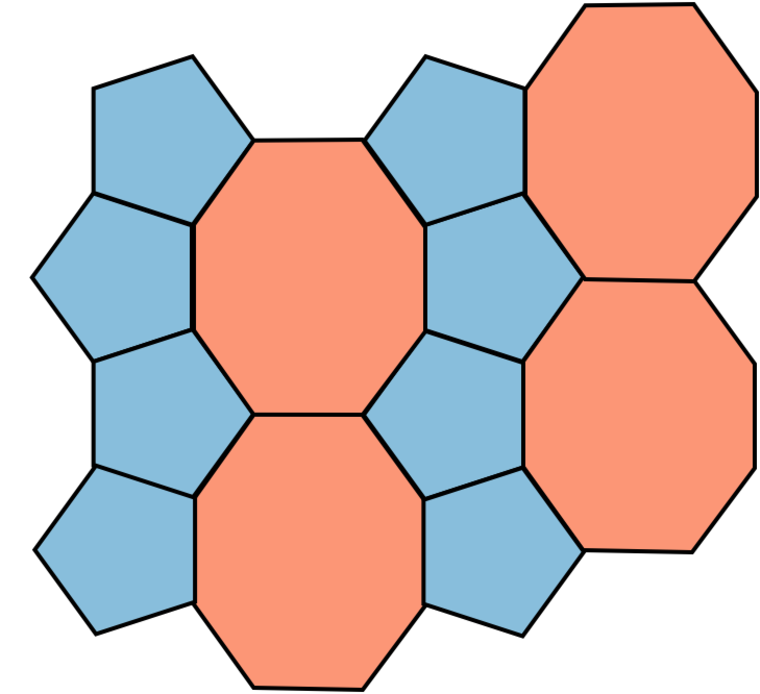
\includegraphics[width=\textwidth]{./appendices/figures/crystal_8_60_52.pdf}
         \caption{$8 - 6^0 - 5^2$, \\$r=-0.350$}
         \label{appfig:86052}
     \end{subfigure}
     \hfill
      \begin{subfigure}[b]{0.15\textwidth}
         \centering
         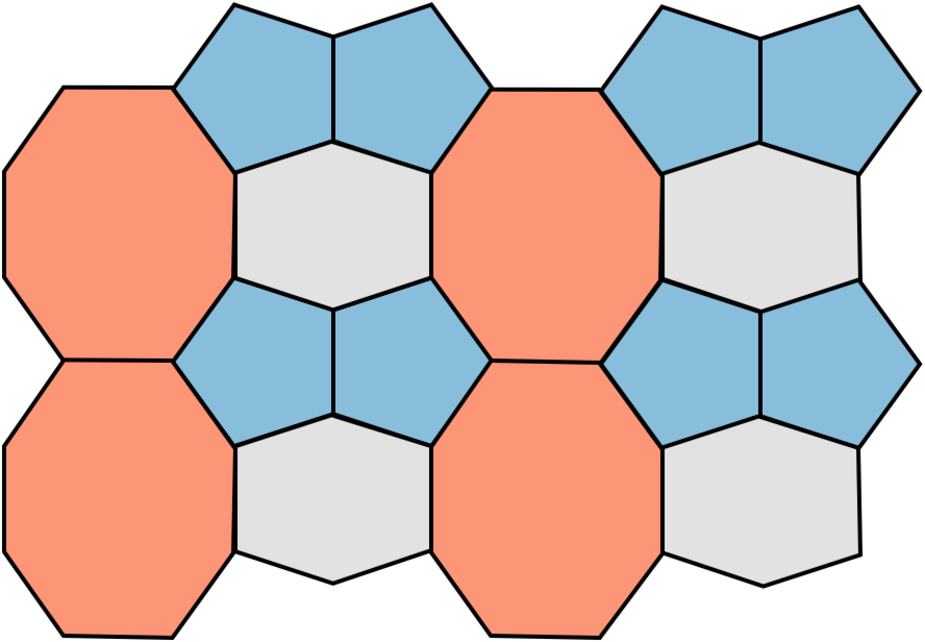
\includegraphics[width=\textwidth]{./appendices/figures/crystal_8_61_52.pdf}
         \caption{$8 - 6^1 - 5^2$, \\$r=-0.185$}
         \label{appfig:86152}
     \end{subfigure}
     \hfill
      \begin{subfigure}[b]{0.15\textwidth}
         \centering
         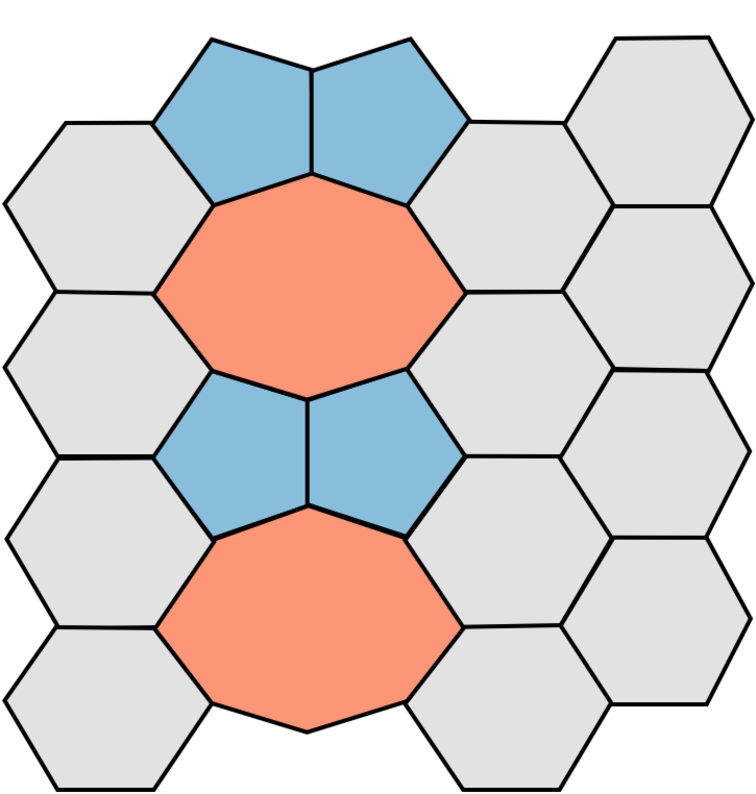
\includegraphics[width=\textwidth]{./appendices/figures/crystal_8_62_52.pdf}
         \caption{$8 - 6^2 - 5^2$, \\$r=-0.373$}
         \label{appfig:86252}
     \end{subfigure}
     \hfill
      \begin{subfigure}[b]{0.15\textwidth}
         \centering
         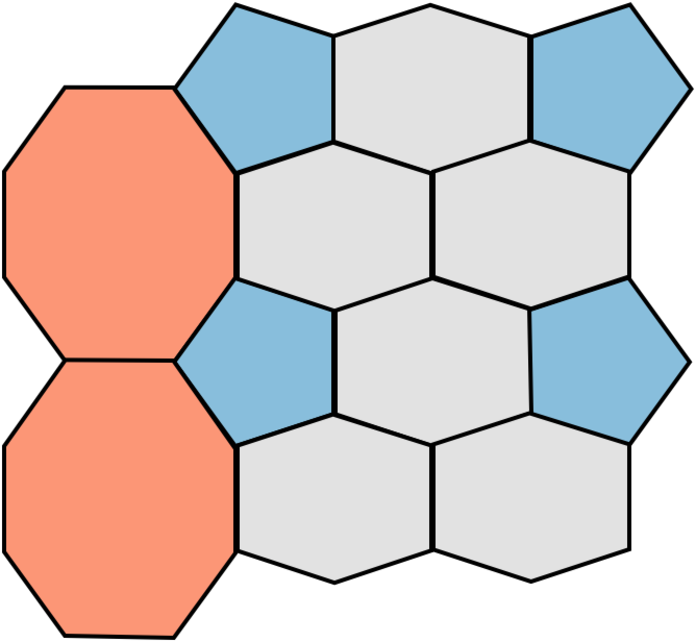
\includegraphics[width=\textwidth]{./appendices/figures/crystal_8_63_52.pdf}
         \caption{$8 - 6^3 - 5^2$, \\$r=-0.220$}
         \label{appfig:86352}
     \end{subfigure}
     \hfill     
     
     \vspace{2mm}
      \begin{subfigure}[b]{0.15\textwidth}
         \centering
         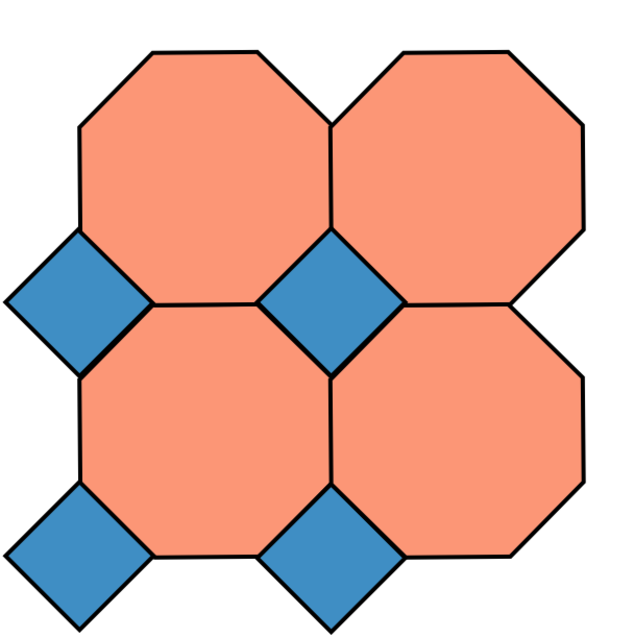
\includegraphics[width=\textwidth]{./appendices/figures/crystal_8_60_4.pdf}
         \caption{$8 - 6^0 - 4$, \\$r=-0.500$}
         \label{appfig:8604}
     \end{subfigure}
     \hfill
      \begin{subfigure}[b]{0.15\textwidth}
         \centering
         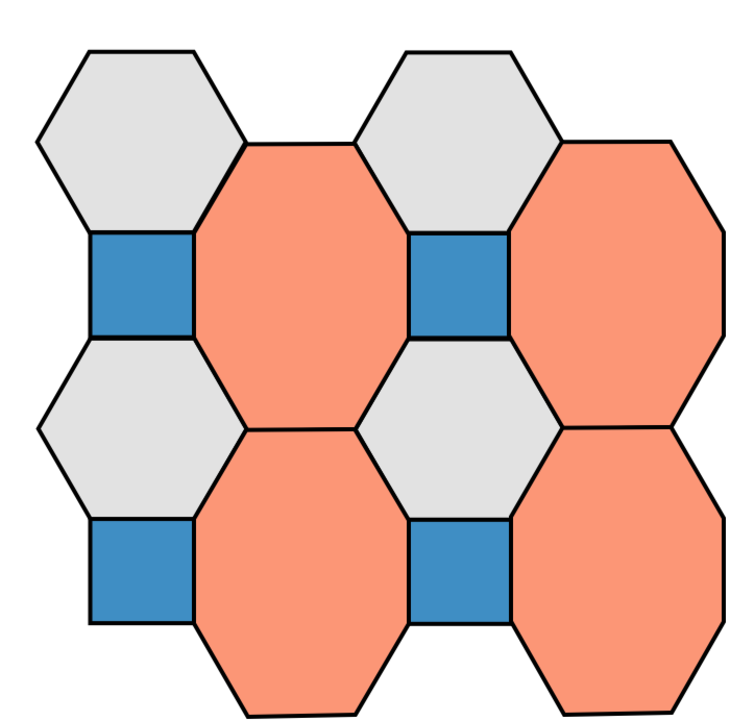
\includegraphics[width=\textwidth]{./appendices/figures/crystal_8_61_4.pdf}
         \caption{$8 - 6^1 - 4$, \\$r=-0.260$}
         \label{appfig:8614}
     \end{subfigure}
     \hfill
      \begin{subfigure}[b]{0.15\textwidth}
         \centering
         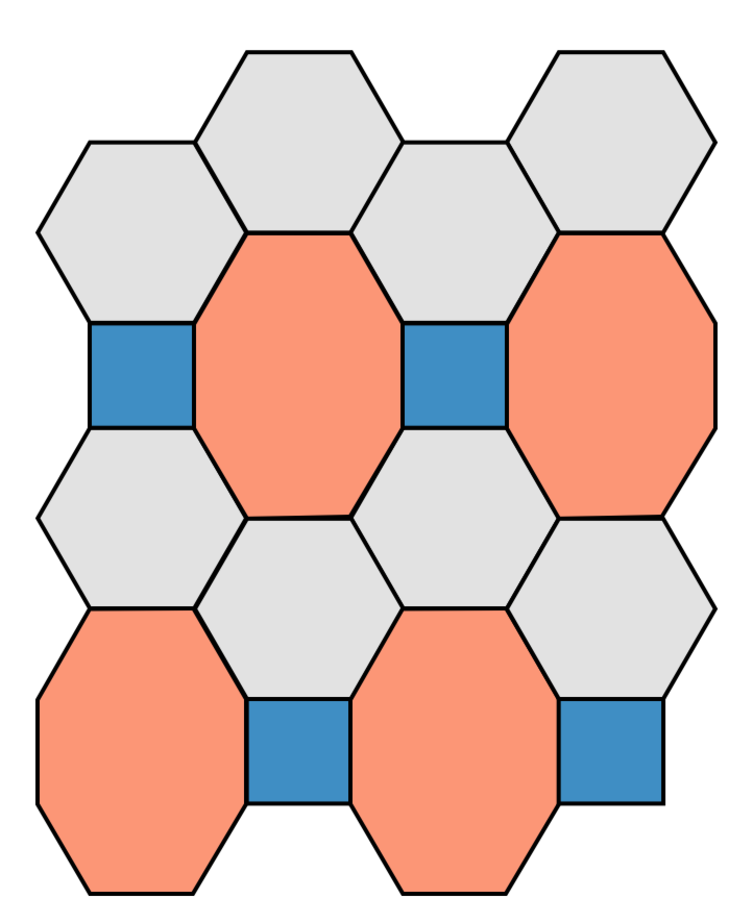
\includegraphics[width=\textwidth]{./appendices/figures/crystal_8_62_4.pdf}
         \caption{$8 - 6^2 - 4$, \\$r=-0.412$}
         \label{appfig:8624}
     \end{subfigure}
     \hfill
      \begin{subfigure}[b]{0.15\textwidth}
         \centering
         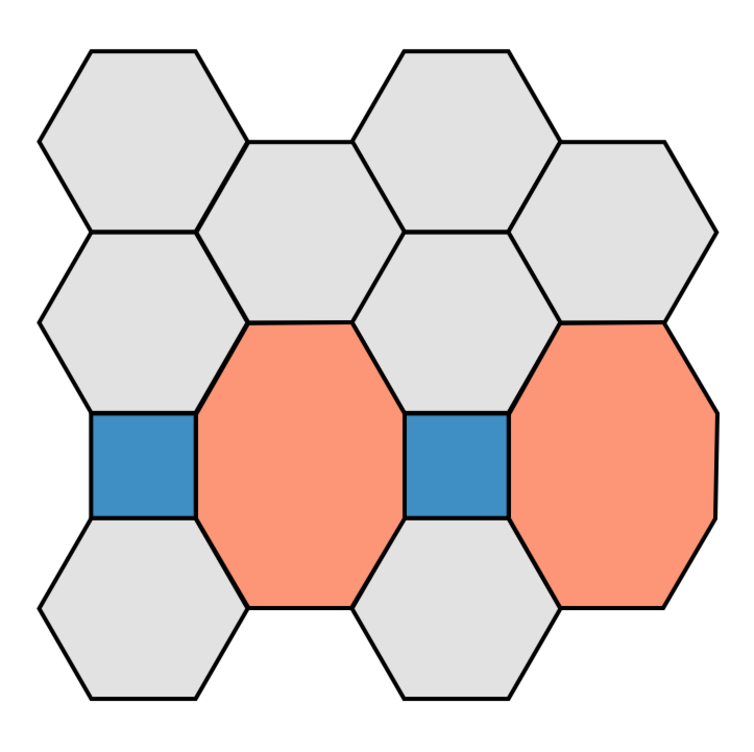
\includegraphics[width=\textwidth]{./appendices/figures/crystal_8_63_4.pdf}
         \caption{$8 - 6^3 - 4$, \\$r=-0.395$}
         \label{appfig:8634}
     \end{subfigure}
     \hfill
     
	
     \caption{Repeating units from two series of crystalline motifs and their assortativities.
      Panels (a)\--(d) show the series $8-6^i-5^2$ with half the number of 8\-- as 5\--rings, interspersed with varying numbers of 6\--rings. Panels (e)\--(h) show the series $8-6^i-4$ with equal numbers of 8\-- and 4\--rings, interspersed with varying numbers of 6\--rings.}
     \label{appfig:crystals}
\end{figure}

\resumetocwriting